\documentclass{beamer}
\usepackage[utf8]{inputenc}
\usepackage[style=ieee]{biblatex}
\addbibresource{paper.bib}
\usepackage{amsmath,amssymb}
\usepackage{utopia} %font utopia imported

\usetheme{Madrid}
\usecolortheme{default}

%------------------------------------------------------------
%This block of code defines the information to appear in the
%Title page
\title[BD recognition] %optional
{Automatic Recognition of Bipolar Disorder from Multimodal Data}

% \subtitle{}

\author[Ziheng Zhang (zz362)] % (optional)
{Ziheng Zhang (zz362@cam.ac.uk)}

\date[21st June, 2019] % (optional)
{21st June, 2019}

%End of title page configuration block
%------------------------------------------------------------



%------------------------------------------------------------
%The next block of commands puts the table of contents at the 
%beginning of each section and highlights the current section:

\AtBeginSection[]
{
  \begin{frame}
    \frametitle{Table of Contents}
    \tableofcontents[currentsection]
  \end{frame}
}
%------------------------------------------------------------


\begin{document}

%The next statement creates the title page.
\frame{\titlepage}


%---------------------------------------------------------
%This block of code is for the table of contents after
%the title page
\begin{frame}
\frametitle{Table of Contents}
\tableofcontents
\end{frame}
%---------------------------------------------------------


\section{Motivation}

\begin{frame}{Bipolar Disorder}

Bipolar Disorder is a serious mental disorder.
\begin{itemize}
    \item BD is associated with significant mortality risk.
    \item 3.9\% of US population are affected by BD in some point of their lives.
\end{itemize}

{
\centering
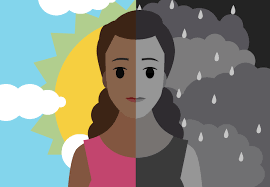
\includegraphics[width=4cm]{images/bd.png}
}

Automatic recognition systems of BD can help early detection of BD symptoms and reduce the treatment resistance. Moreover, it could assist psychologists during the face-to-face interviews.

\end{frame}

\begin{frame}{Bipolar Disorder Corpus}

The Turkish Audio-Visual Bipolar Disorder Corpus
\begin{itemize}
\item was introduced in 2018 
\item consists of audio-visual recordings of interview sessions
\item aims to help develop automatic recognition system
\end{itemize}

Audio/Visual Emotion Challenge (AVEC) 2018 introduces a challenge on the BD recognition from multimodal data based on the BD corpus. 

\end{frame}




\section{Proposed Framework}

\begin{frame}{Proposed Framework}

\begin{figure}[ht]
    \centering
    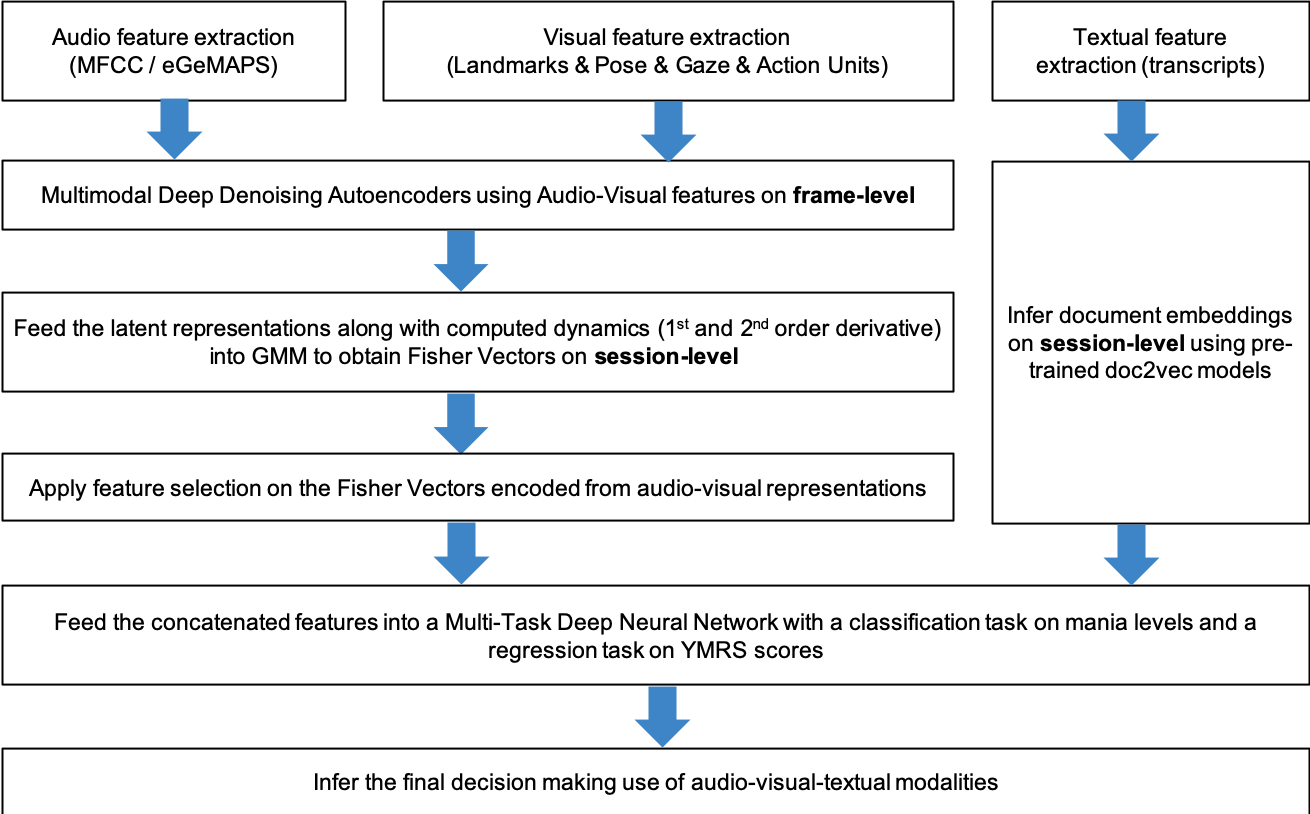
\includegraphics[width=10cm]{images/general_pipeline.png}
    \caption{Pipeline of proposed architecture}
    \label{fig:pipeline}
\end{figure}

\end{frame}

\section{Audio-Visual Modality}

\begin{frame}{Unimodal Deep Denoising Autoencoders}

\begin{figure}[ht]
    \centering
    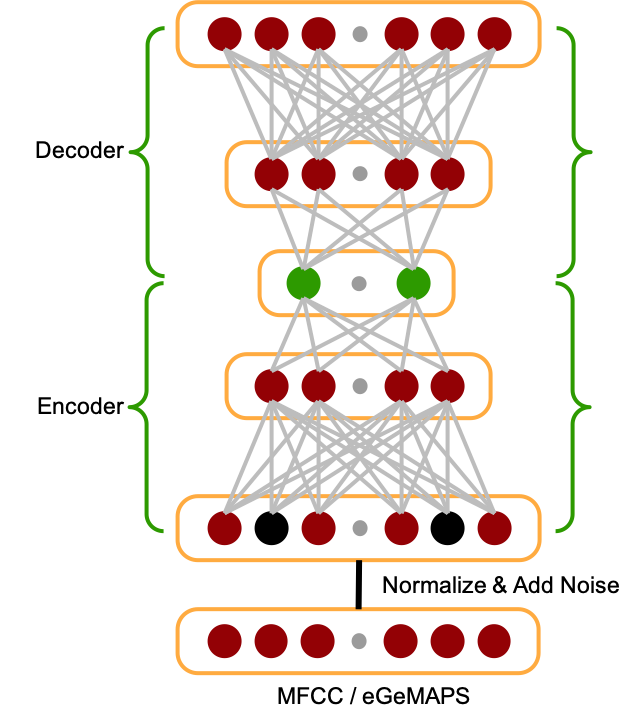
\includegraphics[height=6cm]{images/unimodal_ae_A.png}
    \caption{Unimodal Deep Denoising Autoencoders}
    \label{fig:unimodal}
\end{figure}

\end{frame}

\begin{frame}{Bimodal Deep Denoising Autoencoders}

\begin{columns}

\column{0.7\textwidth}
\begin{figure}[ht]
    \centering
    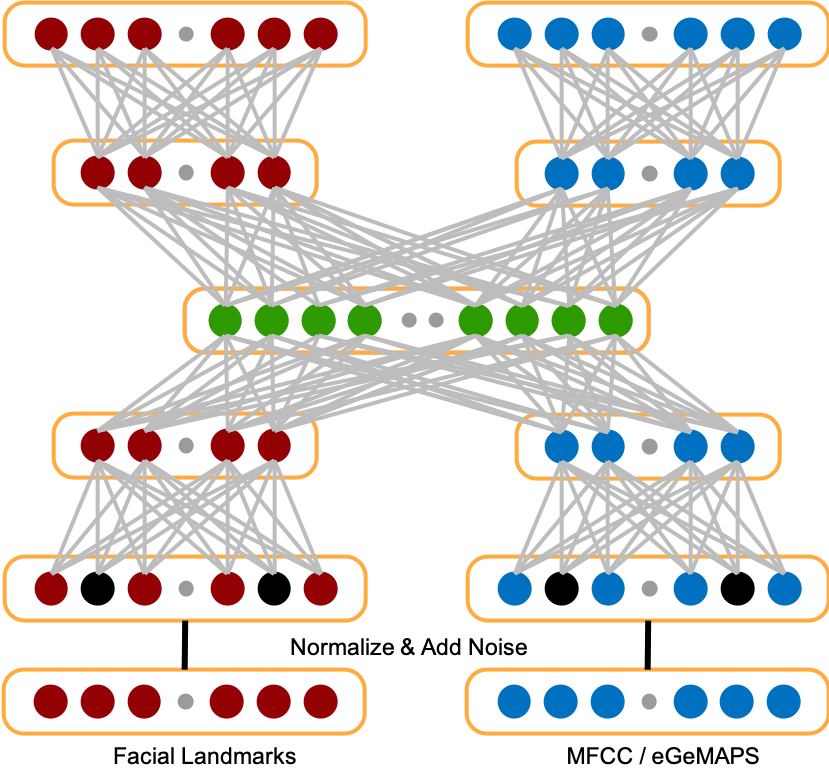
\includegraphics[height=6cm]{images/bimodal_ae.png}
    \caption{Bimodal Deep Denoising Autoencoders}
    \label{fig:bimodal}
\end{figure}

\column{0.3\textwidth}

Two acoustic features are investigated: MFCC or eGeMAPS features.

\end{columns}


\end{frame}

\begin{frame}{Multimodal Deep Denoising Autoencoders}

\begin{figure}[ht]
    \centering
    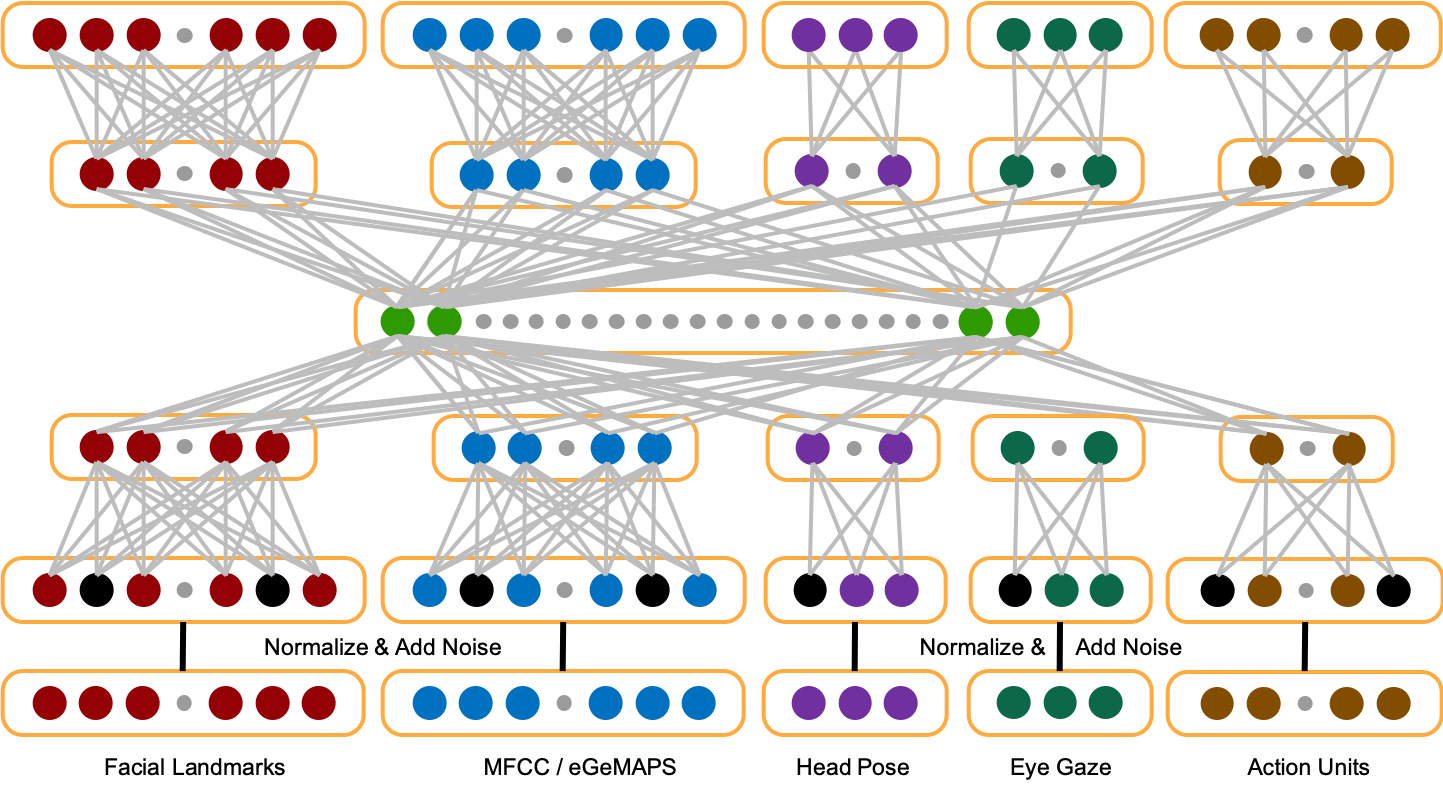
\includegraphics[height=6cm]{images/multimodal_ae.png}
    \caption{Multimodal Deep Denoising Autoencoders}
    \label{fig:multimodal}
\end{figure}

\end{frame}


\section{Textual Modality}

\begin{frame}{Document Embeddings}

\begin{figure}
    \centering
    \centering
    \begin{minipage}{0.55\textwidth}
        \centering
        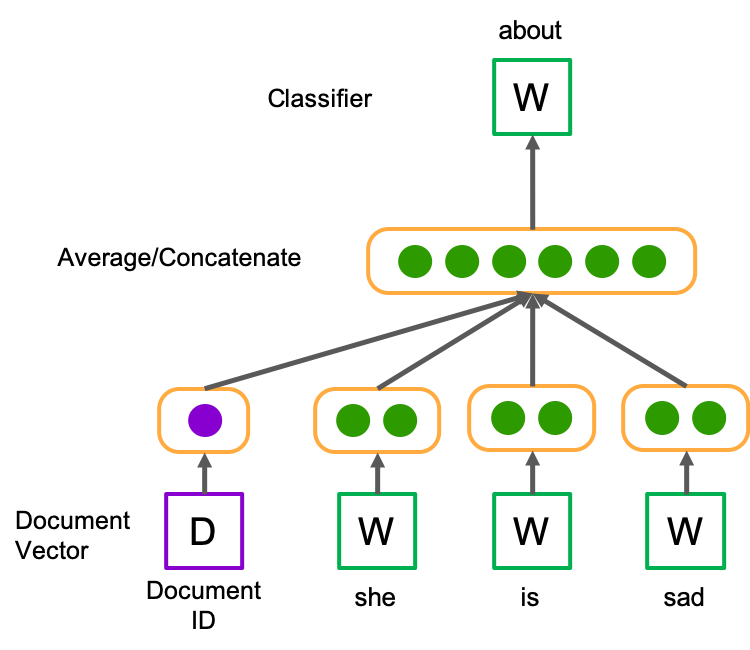
\includegraphics[height=4.6cm]{images/doc2vec_dm-m.png} \\
        (a) doc2vec-DM
    \end{minipage}
    \begin{minipage}{0.43\textwidth}
        \centering
        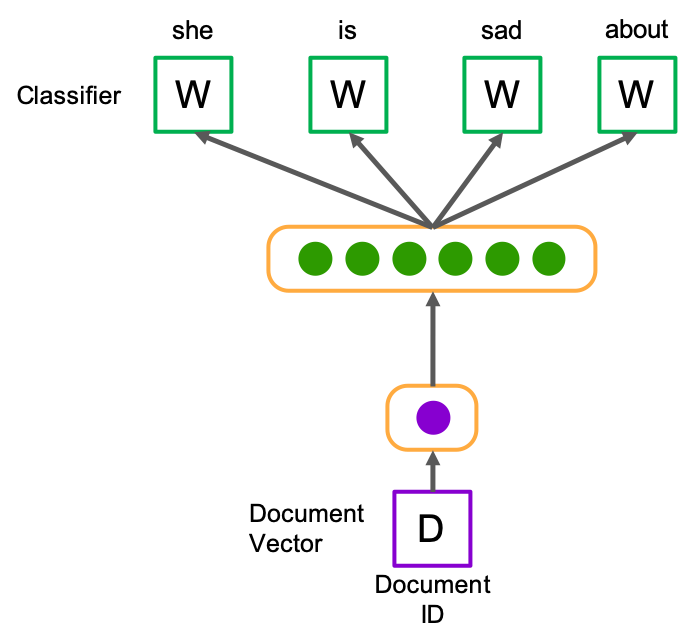
\includegraphics[height=4.6cm]{images/doc2vec_dbow.png} \\
        (b) doc2vec-DBOW
    \end{minipage}
    \caption{Paragraph Vector architectures}
    \label{fig:doc2vec}
\end{figure}

The multimodal framework also utilizes the textual modality, transcripts of interview sessions.
    
\end{frame}


\section{Experimental results}



\begin{frame}{Baseline}

\begin{table}[htb]
    \small
    \centering
    \caption{Baseline systems with Random Forest classifiers on baseline features}
    \begin{tabular}{l|p{1.5cm}|p{1.9cm}|p{1.5cm}|p{1.5cm}|p{1.5cm}}
    \hline
    \hline
         Metric  & MFCC  & eGeMAPS & BoAW & FAU  & BoVW \\
         \hline
         UAR (F) & 0.414 & 0.396 & 0.443 & -     & 0.452 \\
         UAR (S) & 0.413 & 0.455 & \textbf{0.489} & 0.481 & 0.452 \\
         UAP     & 0.410 & 0.370 & 0.439 & \textbf{0.528} & 0.445 \\
         F1      & 0.411 & 0.408 & 0.463 & \textbf{0.503} & 0.448 \\
    \hline
    \hline
    \end{tabular}
    \label{tab:baseline}
\end{table}

The baseline systems do not take into account temporary information and the correlation across modality.

\end{frame}


\begin{frame}{Multimodal Feature Learning}

\begin{table}[htb]
    \small
    \centering
    \caption{Comparison of proposed Multimodal DDAE architectures (selected experimental results)}
    \begin{tabular}{p{1.7cm}|p{1.2cm}|l|p{1.1cm}|l|l|l}
    \hline
    \hline
        Acoustic feature & Hidden ratio & Noise & GMM kernel & UAR & UAP & F1 \\
        \hline
        MFCC  & 0.4 & 0.1 & 32 & \textbf{0.656} & \textbf{0.678} & \textbf{0.667} \\
        \hline
        eGeMAPS & 0.5 & 0.1 & 32 & \textbf{0.622} & \textbf{0.665} & \textbf{0.642} \\
        \hline
        \multicolumn{4}{l|}{Baseline (BoAW)} & 0.489 & 0.439 & 0.463 \\
        \multicolumn{4}{l|}{Baseline (FAU)} & 0.481 & 0.528 & 0.503 \\
        \hline
        \multicolumn{4}{l|}{Best Unimodal DDAE (Landmarks)} & 0.624 & 0.692 & 0.656 \\
        \multicolumn{4}{l|}{Best Unimodal DDAE (MFCC)} & 0.587 & 0.611 & 0.599 \\
        \multicolumn{4}{l|}{Best Unimodal DDAE (eGeMAPS)} & 0.632 & 0.654 & 0.637 \\
        \hline
        \multicolumn{4}{l|}{Best Bimodal DDAE (MFCC)} & 0.656 & 0.677 & 0.666 \\
        \multicolumn{4}{l|}{Best Bimodal DDAE (eGeMAPS)} & 0.566 & 0.611 & 0.587 \\
    \hline
    \hline
    \end{tabular}
    \label{tab:multimodal_res}
\end{table}

\end{frame}



\begin{frame}{Document Embeddings}


\begin{table}[htb]
\centering
\small
\caption{Comparison of proposed document embeddings on the transcripts (selected experimental results)}
    \begin{tabular}{l|p{1.0cm}|p{1.2cm}|p{1.3cm}|l|l|l}
    \hline
    \hline
        Model & Vector size & Window size & Negative words & UAR & UAP & F1 \\
        \hline
        PV-DM & 50 & 10 & 5 & 0.492 & 0.481 & 0.486 \\
        \hline
        PV-DBOW & 50 & - & 5 & 0.505 & 0.544 & 0.524 \\
        \hline
        \multicolumn{4}{l|}{Baseline (BoAW)} & 0.489 & 0.439 & 0.463 \\
        \multicolumn{4}{l|}{Baseline (FAU)} & 0.481 & 0.528 & 0.503 \\
   \hline
   \hline
\end{tabular}
\label{tab:doc2vec_res}
\end{table}
    
\end{frame}

\begin{frame}{Visualization}
    
\begin{figure}[htb]
    \centering
    \small
    \begin{minipage}[c]{0.4\linewidth}
    \centering
    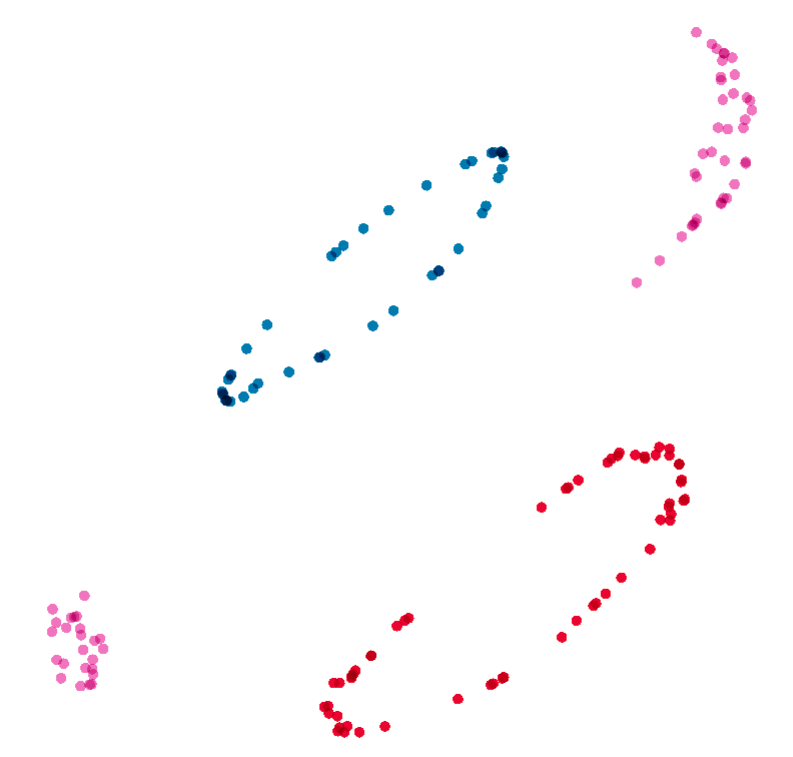
\includegraphics[height=2.5cm]{images/multi_DDAE_MFCC_tsne.png} \\
    (a) multi-DDAE on MFCC
    \end{minipage}
    \begin{minipage}[c]{0.4\linewidth}
    \centering
    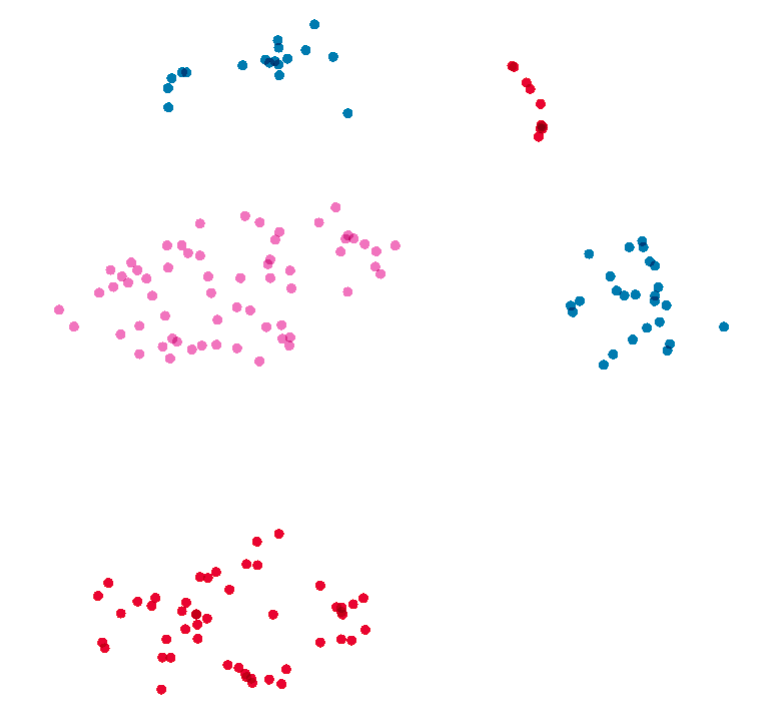
\includegraphics[height=2.5cm]{images/multi_DDAE_eGeMAPS_tsne.png} \\
    (b) multi-DDAE on eGeMAPS
    \end{minipage}
    \\
    \begin{minipage}[c]{0.4\linewidth}
    \centering
    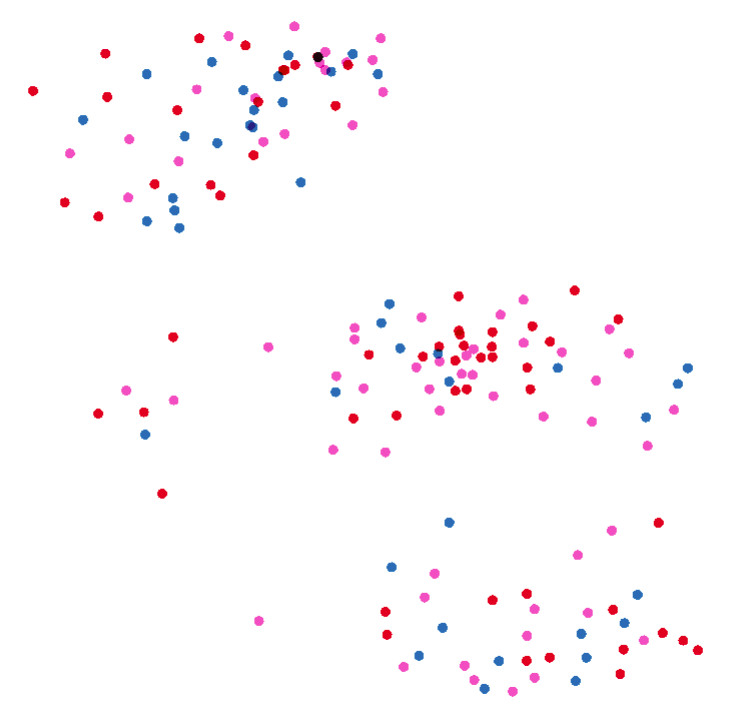
\includegraphics[height=2.5cm]{images/dm_tsne_2d.png} \\
    (c) PV-DM 
    \end{minipage}
    \begin{minipage}[c]{0.4\linewidth}
    \centering
    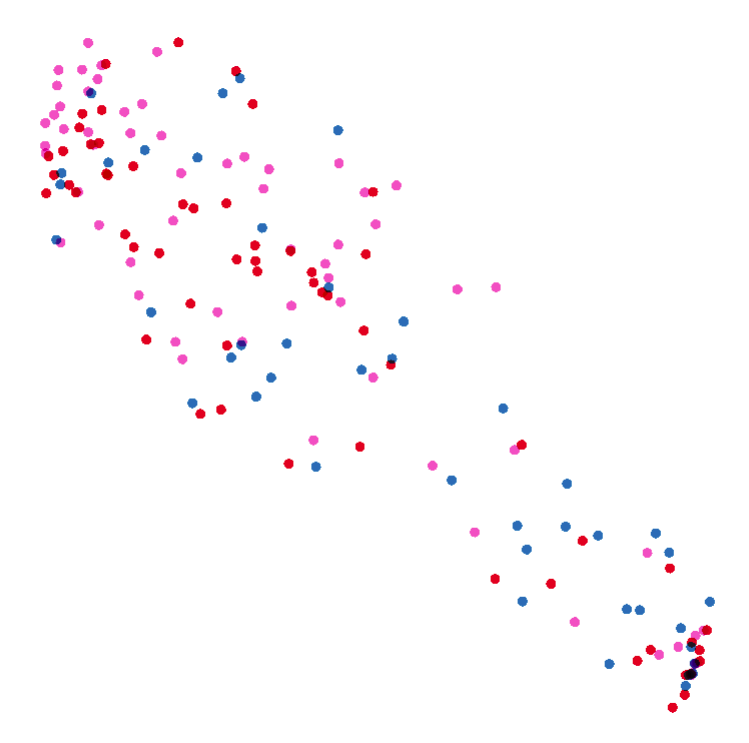
\includegraphics[height=2.5cm]{images/dbow_tsne_2d.png} \\
    (d) PV-DBOW
    \end{minipage}
    \caption{Visualization of Fisher vectors and document embeddings in 2D space using t-SNE algorithm}
    \label{fig:tsne_DDAEs}
\end{figure}

\end{frame}

\begin{frame}{Comparison with competing frameworks in AVEC2018}

After feature fusion, a Multi-Taks neural network is implemented for classification, which makes use of regression task to address the overfitting issues.

\begin{table}[h]
    \small
    \centering
    \caption{Comparison with proposed frameworks in AVEC2018}
    \begin{tabular}{l|l|l}
    \hline
    \hline
        Framework & UAR (dev) & Accuracy (dev) \\
        \hline
        Yang \textit{et al.} 2018 & 0.714 & 0.717 \\
        \hline
        Du \textit{et al.} 2018 & 0.651 & 0.650 \\
        \hline
        Xing \textit{et al.} 2018 & 0.868 & NA \\
        \hline
        Syed \textit{et al.} 2018 & 0.635 & NA \\
        \hline
        \textbf{This work} & \textbf{0.709} & \textbf{0.717} \\
    \hline
    \hline
    \end{tabular}
    \label{tab:avec2018_compare}
\end{table}
    
\end{frame}


\begin{frame}{Generalization}


\begin{figure}[htb]
    \centering
    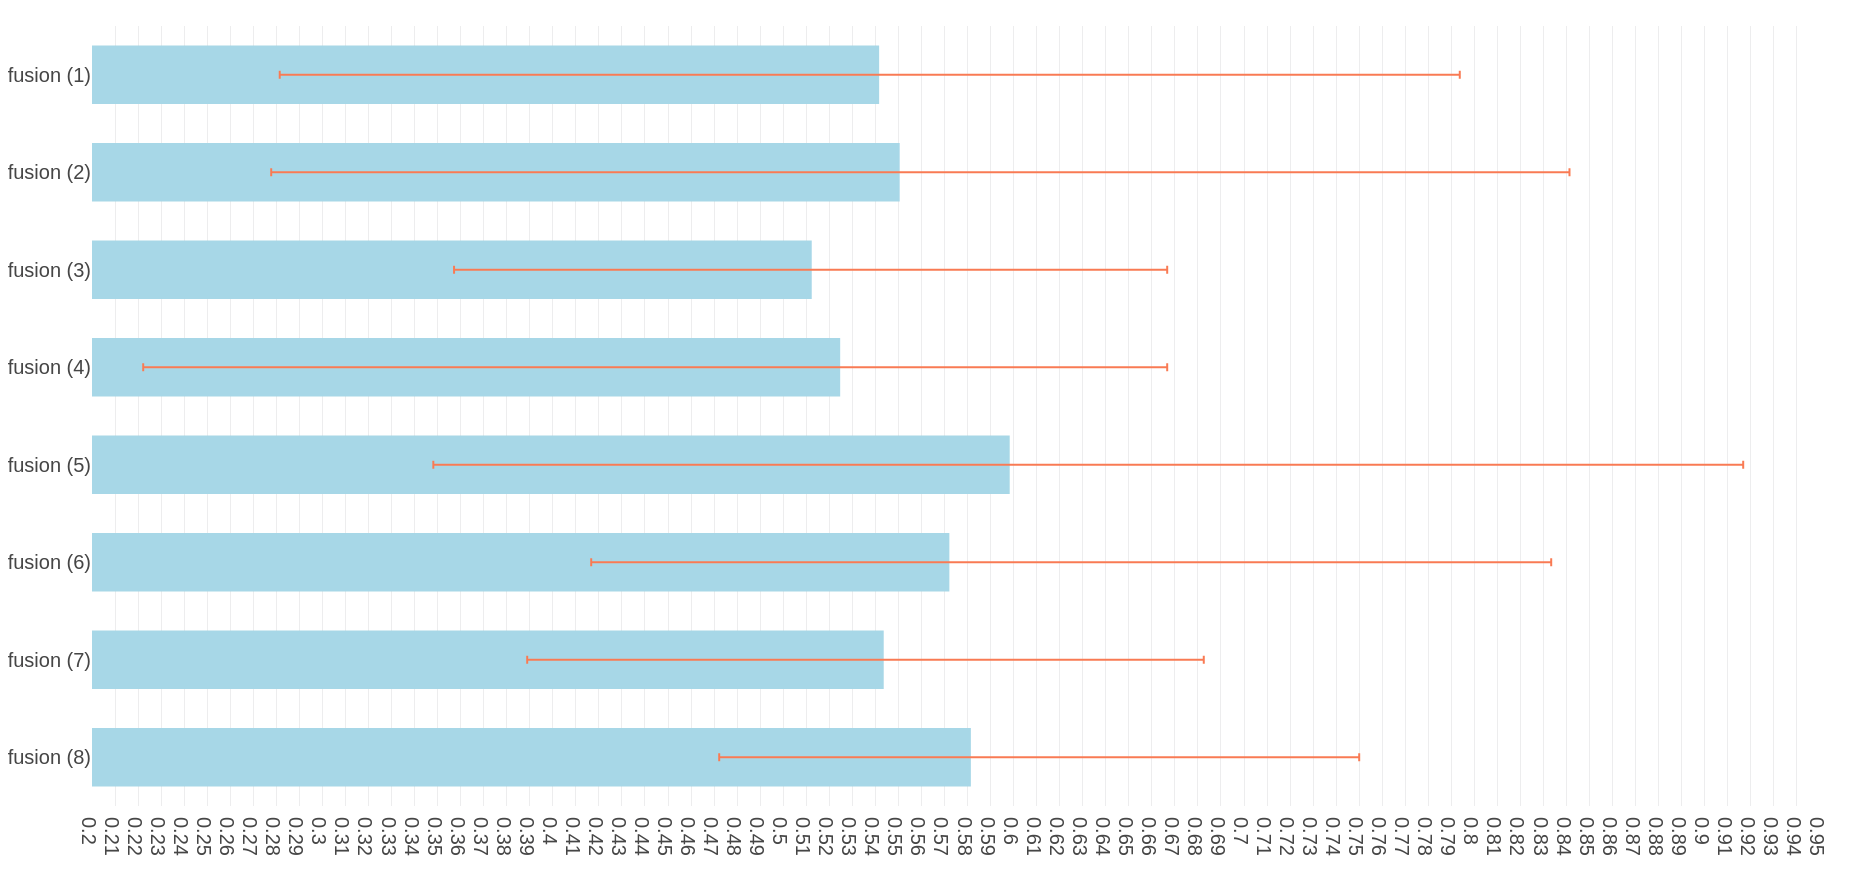
\includegraphics[width=\textwidth]{images/barchart_cv.png}
    \caption{Barchart of the averaged UAR and variance via a 10-fold cross-validation on different fusion frameworks}
    \label{fig:errorbar}
\end{figure}

\end{frame}


\section{Conclusion}

\begin{frame}{Conclusion}

\begin{itemize}
    \item The proposed multimodal framework demonstrates effective in learning the shared representations across modalities while managing the discrepancy.
    \item It achieves the state-of-the-art performance when compared with competing frameworks in the BD recognition task proposed in AVEC2018.
\end{itemize}

\end{frame}

\begin{frame}{Future Work}

\begin{itemize}
    \item To introduce more layers in Deep Denoising Autoencoders to capture the spatial information (like Convolutional layers).
    \item To correlate and decouple different modalities via a semantic interface to obtain more robust representations.
    \item To evaluate the performance of the proposed framework on other similar problems, like the recognition of human state-of-mind proposed in AVEC2019.
\end{itemize}
    
\end{frame}


\begin{frame}
\printbibliography
\end{frame}

\begin{frame}{}
\centering
Thank you for your attention
\end{frame}



\end{document}